\begin{figure}[t]
\setlength{\abovecaptionskip}{5pt plus 3pt minus 2pt}
\setlength{\belowcaptionskip}{-20pt plus 3pt minus 2pt}

\centering
\begin{minipage}[b]{0.52\linewidth}
    \centering
    \includegraphics[width=\textwidth,height=3cm]{./images/football_results.pdf}
    \caption{Results on the KTH Multi-view Football II dataset~\cite{footballDS}, in occluded and blurry scenes with dynamic cameras.
    %Motion reconstruction on the KTH Multi-view Football II dataset~\cite{footballDS} in occluded and blurry scenes. 
    %Each row depicts three views of one time frame. 
    %To the right of each image we put a reconstructed rig of the player. % \#20. 
    %The KTH dataset is filmed using moving cameras, hence camera extrinsic parameters vary between frames. 
    %FLEX is ep-free, so it is agnostic to camera parameters and is not affected by the change in their values.
    }
    \label{fig:football_teaser}
\end{minipage}
\hfill
\begin{minipage}[b]{0.44\linewidth}
    \centering
    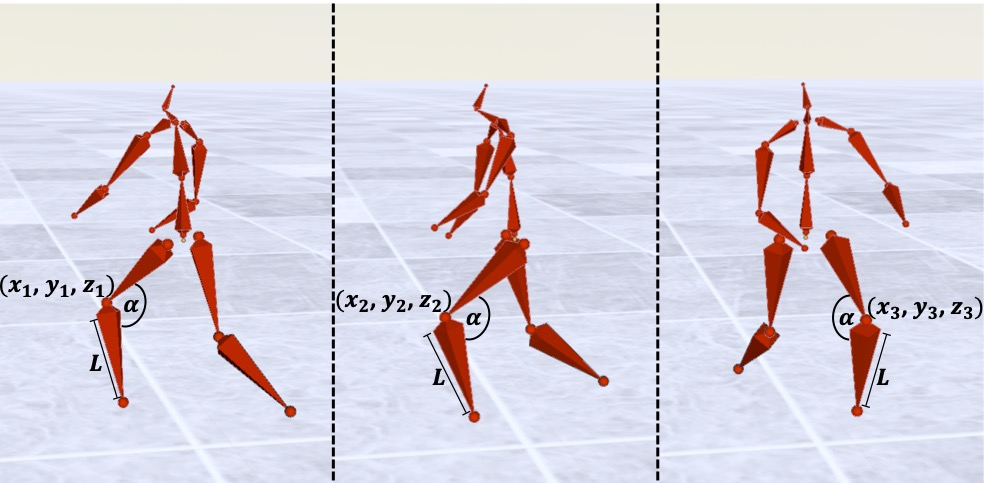
\includegraphics[width=\textwidth,height=3cm]{./images/Skeleton_angles.jpg}
    \caption{3D locations vary across axis systems while 3D rotation angles and bone lengths remain identical.
    %Human rigs observed via the relative axis systems of three cameras. 3D locations vary across axis systems while 3D rotation angles (illustrated with a 2D symbol) and bone lengths remain identical. Thus, fusing the former requires acquaintance of camera parameters while fusing the latter requires none. 
    }
    \label{fig:skeleton_angles}
\end{minipage}
\end{figure}
